\documentclass[10pt]{article}
\usepackage[utf8]{inputenc}
\usepackage[T1]{fontenc}
\usepackage{amsmath}
\usepackage{amsfonts}
\usepackage{amssymb}
\usepackage[version=4]{mhchem}
\usepackage{stmaryrd}
\usepackage{graphicx}
\usepackage[export]{adjustbox}
\graphicspath{ {./images/} }
\usepackage{bbold}

\title{Machine Learning Course - CS-433 
 Expectation-Maximization Algorithm }


\author{Martin Jaggi\\
Last updated on: November 28, 2023}
\date{}


\begin{document}
\maketitle
Nov 29, 2023

credits to Mohammad Emtiyaz Khan \& Rüdiger Urbanke

$$
\text { EPFL }
$$

\section*{Motivation}
Computing maximum likelihood for Gaussian mixture model is difficult due to the log outside the sum.

$\max _{\boldsymbol{\theta}} \mathcal{L}(\boldsymbol{\theta}):=\sum_{n=1}^{N} \log \sum_{k=1}^{K} \pi_{k} \mathcal{N}\left(\mathbf{x}_{n} \mid \boldsymbol{\mu}_{k}, \boldsymbol{\Sigma}_{k}\right)$

Expectation-Maximization (EM) algorithm provides an elegant and general method to optimize such optimization problems. It uses an iterative two-step procedure where individual steps usually involve problems that are easy to optimize.

\section*{EM algorithm: Summary}
Start with $\boldsymbol{\theta}^{(1)}$ and iterate:

\begin{enumerate}
  \item Expectation step: Compute a lower bound to the cost such that it is tight at the previous $\boldsymbol{\theta}^{(t)}$ :
\end{enumerate}

$\mathcal{L}(\boldsymbol{\theta}) \geq \underline{\mathcal{L}}\left(\boldsymbol{\theta}, \boldsymbol{\theta}^{(t)}\right)$ and

$\mathcal{L}\left(\boldsymbol{\theta}^{(t)}\right)=\underline{\mathcal{L}}\left(\boldsymbol{\theta}^{(t)}, \boldsymbol{\theta}^{(t)}\right)$.

\begin{enumerate}
  \setcounter{enumi}{1}
  \item Maximization step: Update $\boldsymbol{\theta}$ :
\end{enumerate}

$$
\boldsymbol{\theta}^{(t+1)}=\arg \max _{\boldsymbol{\theta}} \underline{\mathcal{L}}\left(\boldsymbol{\theta}, \boldsymbol{\theta}^{(t)}\right) .
$$

\section*{Concavity of log}
Given non-negative weights $q$ s.t.

$\sum_{k} q_{k}=1$, the following holds for

any $r_{k}>0$ :

$\log \left(\sum_{k=1}^{K} q_{k} r_{k}\right) \geq \sum_{k=1}^{K} q_{k} \log r_{k}$

\section*{The expectation step}
$\log \sum_{k=1}^{K} \pi_{k} \mathcal{N}\left(\mathbf{x}_{n} \mid \boldsymbol{\mu}_{k}, \boldsymbol{\Sigma}_{k}\right) \geq \sum_{k=1}^{K} q_{k n} \log \frac{\pi_{k} \mathcal{N}\left(\mathbf{x}_{n} \mid \boldsymbol{\mu}_{k}, \boldsymbol{\Sigma}_{k}\right)}{q_{k n}}$

with equality when,

$q_{k n}=\frac{\pi_{k} \mathcal{N}\left(\mathbf{x}_{n} \mid \boldsymbol{\mu}_{k}, \boldsymbol{\Sigma}_{k}\right)}{\sum_{k=1}^{K} \pi_{k} \mathcal{N}\left(\mathbf{x}_{n} \mid \boldsymbol{\mu}_{k}, \boldsymbol{\Sigma}_{k}\right)}$

This is not a coincidence.

\section*{The maximization step}
Maximize the lower bound w.r.t. $\boldsymbol{\theta}$.

$\max _{\boldsymbol{\theta}} \sum_{n=1}^{N} \sum_{k=1}^{K} q_{k n}^{(t)}\left[\log \pi_{k}+\log \mathcal{N}\left(\mathbf{x}_{n} \mid \boldsymbol{\mu}_{k}, \boldsymbol{\Sigma}_{k}\right)\right]$

Differentiating w.r.t. $\boldsymbol{\mu}_{k}, \boldsymbol{\Sigma}_{k}^{-1}$, we

can get the updates for $\boldsymbol{\mu}_{k}$ and $\boldsymbol{\Sigma}_{k}$.

$$
\begin{aligned}
\boldsymbol{\mu}_{k}^{(t+1)} & :=\frac{\sum_{n} q_{k n}^{(t)} \mathbf{x}_{n}}{\sum_{n} q_{k n}^{(t)}} \\
\boldsymbol{\Sigma}_{k}^{(t+1)} & :=\frac{\sum_{n} q_{k n}^{(t)}\left(\mathbf{x}_{n}-\boldsymbol{\mu}_{k}^{(t+1)}\right)\left(\mathbf{x}_{n}-\boldsymbol{\mu}_{k}^{(t+1)}\right)^{\top}}{\sum_{n} q_{k n}^{(t)}}
\end{aligned}
$$

For $\pi_{k}$, we use the fact that they sum to 1. Therefore, we add a Lagrangian term, differentiate w.r.t. $\pi_{k}$ and set to 0 , to get the following update:

$$
\pi_{k}^{(t+1)}:=\frac{1}{N} \sum_{n=1}^{N} q_{k n}^{(t)}
$$

\section*{Summary of EM for GMM}
Initialize $\boldsymbol{\mu}^{(1)}, \boldsymbol{\Sigma}^{(1)}, \boldsymbol{\pi}^{(1)}$ and iterate between the $\mathrm{E}$ and $\mathrm{M}$ step, until $\mathcal{L}(\boldsymbol{\theta})$ stabilizes.

\begin{enumerate}
  \item E-step: Compute assignments $q_{k n}^{(t)}$ :
\end{enumerate}

$$
q_{k n}^{(t)}:=\frac{\pi_{k}^{(t)} \mathcal{N}\left(\mathbf{x}_{n} \mid \boldsymbol{\mu}_{k}^{(t)}, \boldsymbol{\Sigma}_{k}^{(t)}\right)}{\sum_{k=1}^{K} \pi_{k}^{(t)} \mathcal{N}\left(\mathbf{x}_{n} \mid \boldsymbol{\mu}_{k}^{(t)}, \boldsymbol{\Sigma}_{k}^{(t)}\right)}
$$

\begin{enumerate}
  \setcounter{enumi}{1}
  \item Compute the marginal likelihood (cost).
\end{enumerate}

$$
\mathcal{L}\left(\boldsymbol{\theta}^{(t)}\right)=\sum_{n=1}^{N} \log \sum_{k=1}^{K} \pi_{k}^{(t)} \mathcal{N}\left(\mathbf{x}_{n} \mid \boldsymbol{\mu}_{k}^{(t)}, \boldsymbol{\Sigma}_{k}^{(t)}\right)
$$

\begin{enumerate}
  \setcounter{enumi}{2}
  \item M-step: Update $\boldsymbol{\mu}_{k}^{(t+1)}, \boldsymbol{\Sigma}_{k}^{(t+1)}, \pi_{k}^{(t+1)}$.
\end{enumerate}

$$
\begin{aligned}
\boldsymbol{\mu}_{k}^{(t+1)} & :=\frac{\sum_{n} q_{k n}^{(t)} \mathbf{x}_{n}}{\sum_{n} q_{k n}^{(t)}} \\
\boldsymbol{\Sigma}_{k}^{(t+1)} & :=\frac{\sum_{n} q_{k n}^{(t)}\left(\mathbf{x}_{n}-\boldsymbol{\mu}_{k}^{(t+1)}\right)\left(\mathbf{x}_{n}-\boldsymbol{\mu}_{k}^{(t+1)}\right)^{\top}}{\sum_{n} q_{k n}^{(t)}} \\
\pi_{k}^{(t+1)} & :=\frac{1}{N} \sum_{n} q_{k n}^{(t)}
\end{aligned}
$$

If we let the covariance be diagonal i.e. $\boldsymbol{\Sigma}_{k}:=\sigma^{2} \mathbf{I}$, then EM algorithm is same as K-means as $\sigma^{2} \rightarrow 0$.
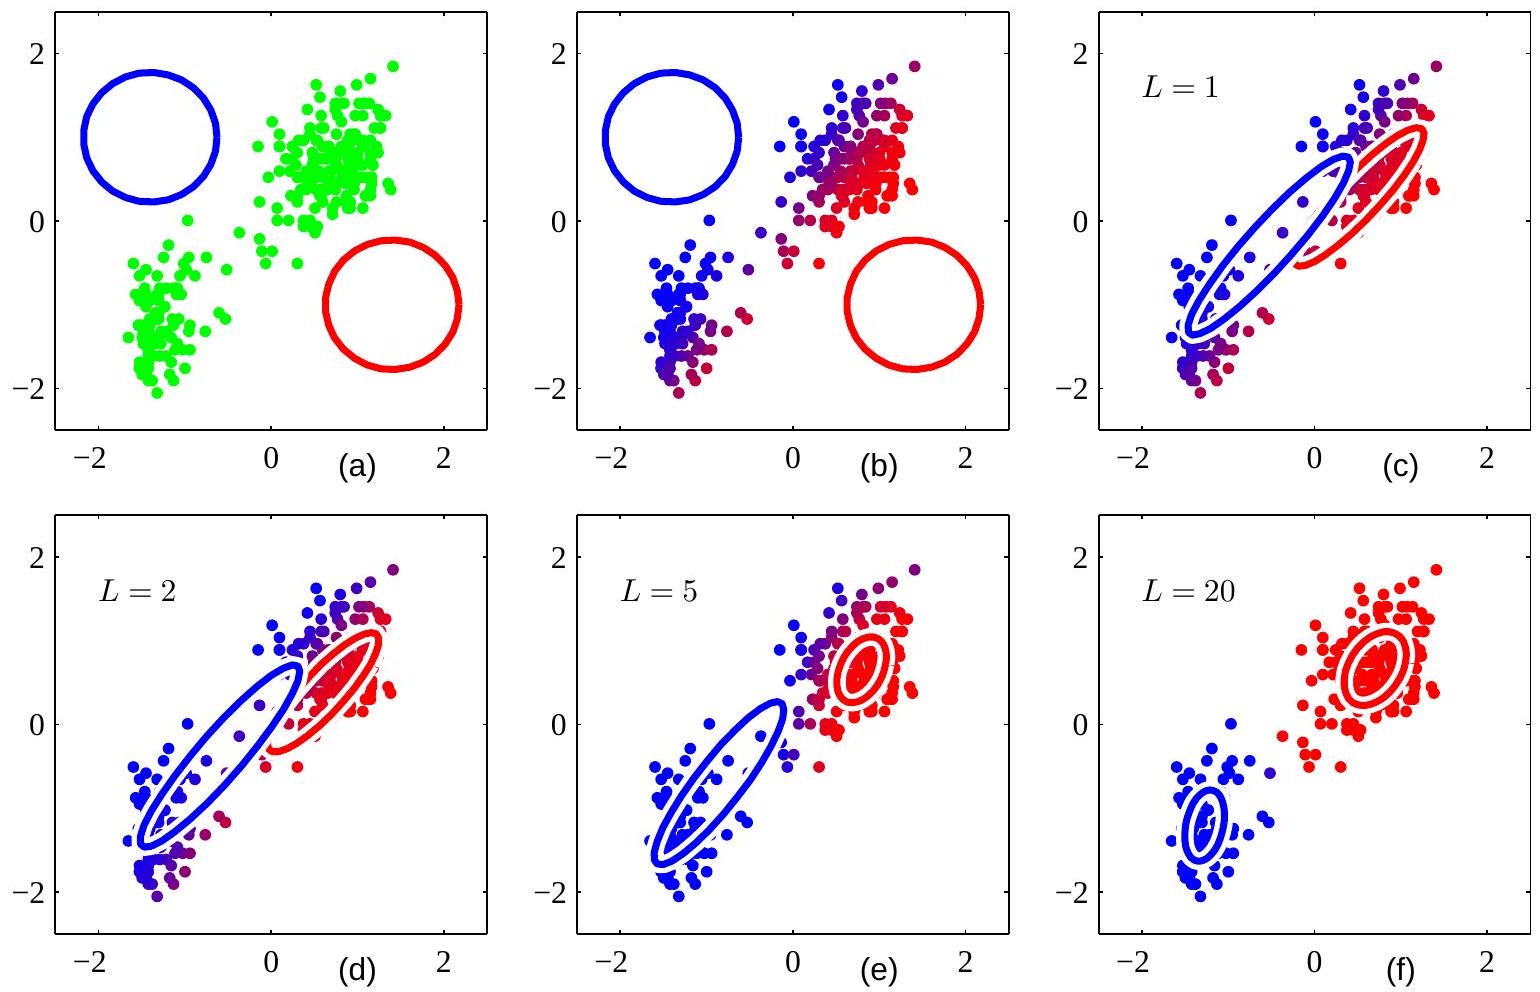
\includegraphics[max width=\textwidth, center]{2023_12_30_e61a87dc872584e254f7g-6(1)}

Figure 1: EM algorithm for GMM

\section*{Posterior distribution}
We now show that $q_{k n}^{(t)}$ is the pos-

terior distribution of the latent vari-

able, i.e. $q_{k n}^{(t)}=p\left(z_{n}=k \mid \mathbf{x}_{n}, \boldsymbol{\theta}^{(t)}\right)$

$p\left(\mathbf{x}_{n}, z_{n} \mid \boldsymbol{\theta}\right)=p\left(\mathbf{x}_{n} \mid z_{n}, \boldsymbol{\theta}\right) p\left(z_{n} \mid \boldsymbol{\theta}\right)=p\left(z_{n} \mid \mathbf{x}_{n}, \boldsymbol{\theta}\right) p\left(\mathbf{x}_{n} \mid \boldsymbol{\theta}\right)$

\begin{center}
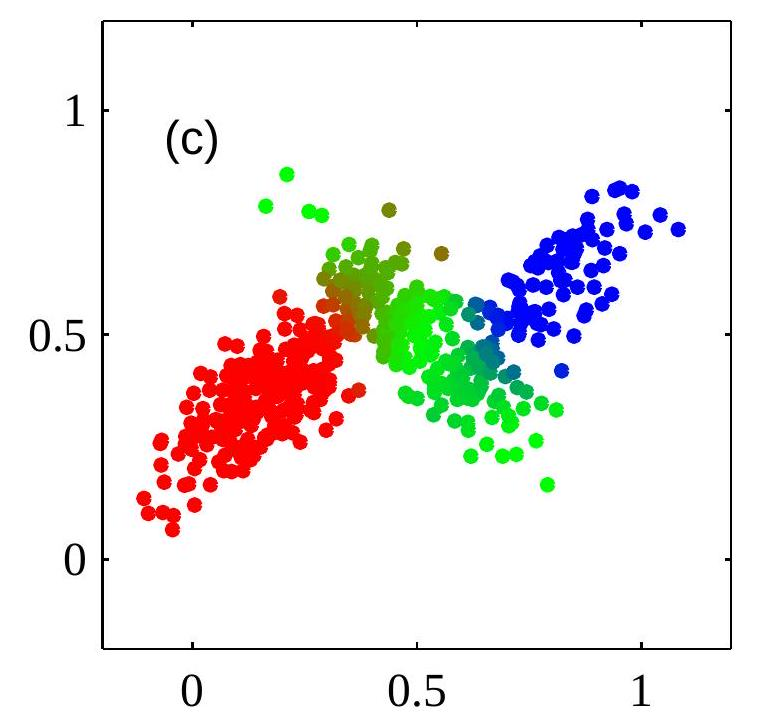
\includegraphics[max width=\textwidth]{2023_12_30_e61a87dc872584e254f7g-6}
\end{center}

\section*{$E M$ in general}
Given a general joint distribution $p\left(\mathbf{x}_{n}, z_{n} \mid \boldsymbol{\theta}\right)$, the marginal likelihood can be lower bounded similarly:

The EM algorithm can be compactly written as follows:

$\boldsymbol{\theta}^{(t+1)}:=\arg \max _{\boldsymbol{\theta}} \sum_{n=1}^{N} \mathbb{E}_{p\left(z_{n} \mid \mathbf{x}_{n}, \boldsymbol{\theta}^{(t)}\right)}\left[\log p\left(\mathbf{x}_{n}, z_{n} \mid \boldsymbol{\theta}\right)\right]$

Another interpretation is that part of the data is missing, i.e. $\left(\mathbf{x}_{n}, z_{n}\right)$ is the "complete" data and $z_{n}$ is missing. The EM algorithm averages over the "unobserved" part of the data.


\end{document}